\documentclass[12pt, a4paper]{article}

% ==========================================
% LANGUAGE & FONT
% ==========================================
\usepackage{fontspec}
\setmainfont{Times New Roman}
\usepackage[english]{babel}
\usepackage{csquotes}           % Required by biblatex with babel

% ==========================================
% PAGE LAYOUT
% Left 3cm, Right 2cm, Top 2cm, Bottom 2cm
% ==========================================
\usepackage[top=2cm, bottom=2cm, left=3cm, right=2cm, headheight=15pt]{geometry}

% ==========================================
% HEADER & FOOTER
% ==========================================
\usepackage{fancyhdr}
\pagestyle{fancy}
\fancyhf{} % Clear default header and footer
\fancyhead[C]{\thepage} % Set page number at top center
\renewcommand{\headrulewidth}{0pt} % Remove header line

% Redefine plain style so that title pages also have the same header
\fancypagestyle{plain}{
  \fancyhf{}
  \fancyhead[C]{\thepage}
  \renewcommand{\headrulewidth}{0pt}
}

% ==========================================
% LINE SPACING
% ==========================================
\usepackage{setspace}
\onehalfspacing

% ==========================================
% FIGURES & TABLES
% ==========================================
\usepackage{graphicx}
\usepackage{booktabs}
\usepackage{multirow}
\usepackage{caption}
\usepackage{subcaption}
\usepackage{float}
\usepackage{tabularx}

% ==========================================
% MATH
% ==========================================
\usepackage{amsmath, amssymb}

% ==========================================
% PLOTS & COLORS
% ==========================================
\usepackage{pgfplots}
\pgfplotsset{compat=1.18}
\usepackage{xcolor}

% ==========================================
% TABLE OF CONTENTS STYLING
% ==========================================
\usepackage{tocloft}            % TOC formatting control
\usepackage{titlesec}           % Section title formatting

% TOC title style
\renewcommand{\cfttoctitlefont}{\large\bfseries}
\renewcommand{\cftaftertoctitle}{\\\rule{\linewidth}{0.4pt}}
\setlength{\cftbeforetoctitleskip}{0pt}
\setlength{\cftaftertoctitleskip}{12pt}

% Section entries in TOC — bold
\renewcommand{\cftsecfont}{\bfseries}
\renewcommand{\cftsecpagefont}{\bfseries}
\renewcommand{\cftsecleader}{\cftdotfill{\cftdotsep}}
\setlength{\cftsecindent}{0pt}
\setlength{\cftsecnumwidth}{2em}
\setlength{\cftbeforesecskip}{6pt}

% Subsection entries in TOC
\renewcommand{\cftsubsecfont}{\normalfont}
\renewcommand{\cftsubsecpagefont}{\normalfont}
\setlength{\cftsubsecindent}{2em}
\setlength{\cftsubsecnumwidth}{2.8em}
\setlength{\cftbeforesubsecskip}{2pt}

% Subsubsection entries in TOC
\setlength{\cftsubsubsecindent}{4.5em}
\setlength{\cftsubsubsecnumwidth}{3.5em}

% Section title formatting in document body
\titleformat{\section}
  {\normalfont\fontsize{13}{15}\bfseries}{\thesection}{1em}{}
\titleformat{\subsection}
  {\normalfont\fontsize{12}{14}\bfseries}{\thesubsection}{1em}{}
\titleformat{\subsubsection}
  {\normalfont\fontsize{12}{14}\itshape}{\thesubsubsection}{1em}{}

% ==========================================
% MISCELLANEOUS
% ==========================================
\usepackage{url}
\usepackage{microtype}          % Improved text justification
\usepackage{parskip}            % Space between paragraphs

% ==========================================
% REFERENCE MANAGEMENT (APA)
% Must be loaded before hyperref
% ==========================================
\usepackage[backend=biber, style=apa, sorting=nyt]{biblatex}
\addbibresource{references.bib}

% ==========================================
% HYPERREF — always load LAST
% ==========================================
\usepackage[
  colorlinks=true,
  linkcolor=black,
  citecolor=blue,
  urlcolor=blue,
  bookmarks=true,
  pdfusetitle
]{hyperref}

\usepackage{tikz}
\usetikzlibrary{shapes.geometric, arrows.meta, positioning, fit}
\usepackage{placeins}

% ==========================================
% RESEARCH PAPER INFORMATION
% ==========================================
\title{
  \textbf{Multimodal A.I: \\
  A Revolution for Enterprise Digital Transformation in Vietnam}
}

\author{
  Nguyễn Đại Quân\texorpdfstring{\textsuperscript{1}}{[1]},
  Nguyễn Phú Nam \texorpdfstring{\textsuperscript{2}}{[2]},
  Trương Hoàng Tùng \texorpdfstring{\textsuperscript{3}}{[3]}
  Nguyễn Dương Hiếu \texorpdfstring{\textsuperscript{4}}{[4]} \\[6pt]
  \small\textit{\texorpdfstring{\textsuperscript{1}}{[1]}Mathematical Economics, National Economics University} \\
}
\date{\today}

% ==========================================
% MAIN BODY
% ==========================================
\begin{document}

\maketitle

% ==========================================
% ABSTRACT
% ==========================================
\begin{abstract}
\noindent
Digital transformation in enterprises has accelerated the adoption of Cognitive Robotic Process Automation (RPA) capable of processing unstructured and multimodal inputs such as documents, images, and speech. However, deploying end-to-end Large Language Models (LLMs) in high-frequency enterprise workflows introduces significant challenges related to prediction accuracy, computational latency, and operational cost.
This study proposes a modular two-stage framework for multimodal information extraction and entity resolution designed for domain-specific enterprise environments. The architecture separates signal interpretation from semantic reasoning. In the first stage, specialized perception modules—including Optical Character Recognition (OCR) and Automatic Speech Recognition (ASR)—convert multimodal inputs into textual representations. In the second stage, a unified Large Language Model performs zero-shot structured entity extraction from the transcribed content.
To resolve extracted entities against large enterprise catalogs, the system employs a hybrid retrieval mechanism that combines dense semantic representations from Sentence-BERT with sparse lexical matching using BM25. The two retrieval signals are integrated through Reciprocal Rank Fusion (RRF) to improve robustness and recall.
Experimental evaluation demonstrates that the proposed system achieves high extraction performance with F1-scores of 0.91 for visual inputs and 0.85 for acoustic inputs under noisy conditions. The hybrid retrieval module maintains a Recall@5 of 0.93 on a catalog containing 50,000 stock-keeping units (SKUs). In addition, the architecture achieves an estimated operational cost of \$13.50 per 1,000 processed documents while limiting the human-in-the-loop intervention rate to 12.5%.
These results indicate that the proposed modular architecture provides an efficient and scalable approach for integrating noisy multimodal inputs into structured enterprise data pipelines.


\medskip
\noindent\textbf{Keywords}: Multimodal Information Extraction, Robotic Process Automation, Large Language Models, Hybrid Retrieval, Entity Resolution, Enterprise Automation.

\medskip
\noindent\textbf{JEL Classification:} O33, L86, M15
\end{abstract}

\newpage

% ==========================================
% TABLE OF CONTENTS (clickable via hyperref)
% ==========================================
{
  \hypersetup{linkcolor=black}   % TOC links in black (professional look)
  \setcounter{tocdepth}{3}       % Show: section / subsection / subsubsection
  \tableofcontents
}

\newpage

% ==========================================
% SECTION FILES
% ==========================================

\section{Introduction}
In the framework of the fourth industrial revolution, Digital Transformation (DX) has become a cornerstone of Vietnam’s national economic strategy. Under the "National Digital Transformation Program to 2025, with a vision to 2030" (Decision No. 749/QD-TTg), the Vietnamese government has set ambitious goals to shift from basic digitization to a comprehensive data-driven digital economy. For enterprises in Vietnam, this transition is no longer merely an option but a critical requirement to optimize operational costs and enhance global competitiveness. As a result, businesses across sectors—from banking to manufacturing—are aggressively integrating advanced technologies to restructure their traditional workflows.

Among these technologies, Robotic Process Automation (RPA) has emerged as a principal mechanism for automation in the Vietnamese market. RPA's ability to handle high-volume, repetitive tasks with speed and precision has made it an attractive entry point for enterprises from SMEs to large enterprises. By deploying software robots to mimic human interactions with digital systems, companies have successfully automated back-office functions such as payroll processing, data entry, and basic reporting.

However, as the DX journey matures, traditional RPA is reaching a significant plateau. The fundamental limitation of RPA lies in its rigid, rule-based nature: these tools are only capable of processing highly structured data (e.g., Excel or SQL databases). In the specific context of Vietnam, this limitation is magnified by several factors:

Dominance of Unstructured Data: A vast majority of business inputs in Vietnam—such as handwritten invoices, scanned delivery notes, and diverse document formats—remain unstructured.

Voice-Based Transactions: Many local SMEs still rely heavily on hand-written invoices, verbal communication and voice-based ordering, which traditional RPA cannot interpret.

Regional Linguistic Nuances: Standard automation tools often struggle with the complexity of Vietnamese dialects and non-standard shorthand in manual records.

When faced with these non-standardized and irregular inputs, traditional RPA workflows fail, necessitating human intervention and negating the benefits of end-to-end automation. To bridge this gap, Multimodal Artificial Intelligence (AI) has emerged as a transformative solution. By integrating computer vision, speech recognition, and natural language processing, Multimodal AI provides RPA with the sensory perception required to handle the complexities of the real-world Vietnamese business environment.

The primary objective of this research is to propose and implement a robust R\&D framework for an "Automated Multimodal Ordering System" specifically engineered for the Vietnamese enterprise ecosystem. Moving beyond the theoretical applications of AI, this paper focuses on the technical synergy between Computer Vision (CV), Automatic Speech Recognition (ASR) and Semantic Information Retrieval (IR) to bridge the gap between unstructured inputs and structured digital procurement records. The research aims to address the following technical challenges:

\begin{enumerate}
    \item \textbf{Architectural Design of a Modular End-to-End Pipeline}: We define a comprehensive system architecture that transforms raw Vietnamese audio signals and hand-written invoices into finalized, schema-compliant digital orders. This involves a decoupled, multi-stage process: from the selection of high-fidelity speech-to-text engines to a post-processing refinement layer and final semantic mapping. By modularizing the pipeline, the system ensures flexibility and ease of maintenance across different enterprise environments.
    \item \textbf{Strategic Model Selection and Phonetic Refinement}: A core focus of this study is the empirical evaluation and selection of Automatic Speech Recognition (ASR) models based on rigorous metrics, including Word Error Rate (WER) and Levenshtein Distance. Rather than intensive fine-tuning, we implement a Cognitive Refinement Layer using Large Language Models (LLMs) to correct common phonetic misinterpretations and dialectal inconsistencies (e.g., misspellings like "bun" for "bulb" or "oát" for "watt"). This heuristic approach significantly enhances transcription reliability in noisy, real-world commercial contexts.
    \item \textbf{Two-Tier Semantic Retrieval and Vector-Based SKU Mapping}: We explore a sophisticated information retrieval strategy that combines \textbf{LLM-based Pre-filtering} with \textbf{Vector Search mechanisms}. The LLM first cleans and extracts core entities—such as product identifiers, quantities, and units—from the refined text. These entities are then mapped against enterprise databases using high-dimensional vector embeddings, ensuring precise product identification (SKU mapping) even when the input contains non-standard terminology or regional jargon. 
\end{enumerate}
\section{Literature Review}

\subsection{The Macro-Context: From Digital Transformation to Cognitive RPA}

\subsubsection{The Imperative of Digital Transformation in the Modern Economy}
Digital transformation represents the foundational restructuring of enterprise operations, characterized by the deep integration of digital technologies to fundamentally alter how value is delivered, measured, and optimized. In the modern economic paradigm, traditional data silos—where distinct departments hoard isolated datasets and operational metrics—are being rapidly dismantled in favor of interconnected, enterprise-wide digital ecosystems \parencite{peng2022digital}. Historically, artificial intelligence systems deployed within corporate infrastructures have focused almost exclusively on single modalities, such as isolated text-mining algorithms utilized for basic sentiment analysis or standalone image-based recognition models tailored for highly specific, narrowly defined manufacturing applications. However, as the scope of computational capabilities has grown, alongside the exponential increase in big data velocity, so has the critical demand for multimodal data interpretation \parencite{sura2025multimodal}.

The massive accumulation of structured data, including deterministic transaction logs, rigid financial records, and tabular customer relationship management databases, occurs concurrently with the generation of vast lakes of unstructured data. This unstructured matrix encompasses nuanced customer reviews, highly variable visual marketing data, dynamic social media content, and continuous communication audio. The coexistence of these heterogeneous data types necessitates a profound transition from reactive, retrospective analytics to proactive, predictive data-driven intelligence \parencite{gumber2025multimodal}. Empirical analyses indicate that the digital transformation of manufacturing and service enterprises plays a significant, positive role in improving overall enterprise performance, primarily by shifting organizational dependence from traditional, constrained production factors to highly scalable data elements \parencite{peng2022digital}.

By seamlessly integrating these diverse and heterogeneous data formats, enterprises can transcend superficial metrics to achieve a significantly more contextual, robust, and holistic understanding of complex market phenomena \parencite{sura2025multimodal}. Furthermore, evidence suggests that digital transformation indirectly improves performance by systematically optimizing operational efficiency and reducing production costs. Through strategic alignment, enterprises that adopt data-driven innovation ecosystems achieve sustained competitive advantages, fundamentally shifting market power and enabling high-quality growth \parencite{khan2025adaptive}. The ability to process unstructured, multimodal inputs acts as a catalyst for breaking through rigid sectoral barriers, promoting internal specialization, and advancing interdepartmental collaboration, which collectively drive a scalable increase in capital return rates and decision-making efficiency.

\subsubsection{The Evolution of Robotic Process Automation}
Initially, enterprise automation was heavily reliant on traditional Robotic Process Automation (RPA)—software systems explicitly designed to execute highly structured, rule-based, and heavily deterministic tasks. While conventional RPA dramatically improved operational efficiency by automating repetitive, high-volume tasks across standardized user interfaces, its utility was strictly bounded by its inherent fragility \parencite{peng2022digital}. Traditional RPA was fundamentally incapable of processing unstructured data, adapting to even minor user interface modifications, or handling cognitive ambiguities. The prerequisite for successful conventional RPA deployment required highly stable environments with perfectly structured input data, devoid of the variations, noise, and unpredictability typical in human-generated content. Consequently, any deviation from pre-programmed logic resulted in process failure, requiring constant manual intervention and maintenance.

As global supply chains, e-commerce networks, and modern financial systems grow increasingly interconnected and complex, organizations require robust automation frameworks capable of nonlinear pattern recognition and high-dimensional data processing. This imperative has catalyzed the evolutionary leap from standard mechanical automation to "Cognitive RPA," wherein advanced artificial intelligence acts as the central, dynamic reasoning engine \parencite{khan2025adaptive}. In this advanced state, software agents transcend the role of mere mechanical tools to act as quasi-human collaborators on core business tasks, actively participating in data analysis, problem diagnosis, and strategic decision-making \parencite{kephart2021multimodal}.

To be highly effective collaborators in modern corporate environments, these sophisticated systems must move far beyond simple text processing to understand complex multi-modal communications. This involves not only transcribing what is said but deeply interpreting speech complemented by vital non-verbal behaviors and contextual cues, such as deictic gestures, eye gaze, and facial expressions during human-machine interactions \parencite{kephart2021multimodal}. For Cognitive RPA to function efficiently and autonomously, the underlying systems must also satisfy rigorous data quality standards, ensuring the completeness, actuality, accuracy, and validity of the ingested unstructured data.

\begin{table}[htbp]
\centering
\caption{Comparison Between Traditional RPA and Cognitive RPA}
\label{tab:rpa_comparison}
\begin{tabularx}{\textwidth}{@{} l >{\raggedright\arraybackslash}X >{\raggedright\arraybackslash}X @{}}
\toprule
\textbf{Attribute} & \textbf{Traditional RPA} & \textbf{Cognitive RPA} \\
\midrule
Primary Data Input & Highly structured (Relational databases, CSVs) & Unstructured and Multimodal (Audio, Images, Free-text) \\
\addlinespace
Execution Paradigm & Deterministic, rule-based, IF-THEN logic & Probabilistic, learning-based, contextual reasoning \\
\addlinespace
Adaptability & Extremely brittle; fails upon UI or data format changes & Highly adaptive; generalizes across varying inputs and noise \\
\addlinespace
Human Interaction & Minimal; operates strictly in the background & Collaborative; interprets complex cues like gaze and gestures \\
\addlinespace
Tech. Foundation & Screen scraping, basic APIs, macros & Deep Neural Networks, Transformers, Multimodal LLMs \\
\addlinespace
Operational Goal & Labor reduction for repetitive, manual keystrokes & Strategic decision support, anomaly detection, predictive forecasting \\
\bottomrule
\end{tabularx}
\end{table}

\subsubsection{The Landscape of Digital Transformation and RPA in Vietnam}
In the distinct context of Vietnam's rapid digital transformation, local enterprises encounter highly specific operational hurdles. Primarily, they face significant barriers stemming from rigid legacy IT infrastructures and the linguistic complexities of the Vietnamese language, which is tonal, monosyllabic, and characterized by limited large-scale training resources \parencite{le2024phowhisper}. Consequently, attempting to directly apply standard, off-the-shelf Western automation tools often results in systemic failures and unacceptably high error rates during data ingestion \parencite{khan2025adaptive}. This critical gap has catalyzed a pressing demand for localized, multimodal RPA systems. Such bespoke systems increasingly leverage advanced self-supervised learning architectures to effectively process the unique noise inherent in Vietnamese enterprise data—including conversational speech heavily laden with bilingual loanwords and unstructured handwritten documents—while achieving high accuracy at a minimal manual annotation cost \parencite{gumber2025multimodal, zhuo2025vietasr}.

The Fourth Industrial Revolution has exerted a profound impact on the socio-economic landscape of Vietnam, driving digital transformation across critical sectors such as finance, banking, and manufacturing. Within this corporate ecosystem, RPA has emerged as a foundational technology. Unlike previous IT overhauls, such as the implementation of massive Enterprise Resource Planning (ERP) systems—which often demanded exorbitant upfront capital and extensive infrastructural modifications—RPA offers a highly agile and cost-effective alternative. In the Vietnamese context, RPA effectively functions as a "virtual employee," interfacing seamlessly between legacy IT systems and back-office processes to execute repetitive human actions at an accelerated pace and with superior accuracy \parencite{chuong2019rpa}.

A 2019 study underscored that the Vietnamese market presents vast opportunities for RPA deployment, particularly in domains characterized by high transaction volumes and labor-intensive workflows \parencite{chuong2019rpa}. In the banking sector, prominent institutions such as Vietinbank have pioneered the use of RPA to navigate stringent operational processes. For instance, card activation teams utilize RPA bots to validate client requests against complex compliance guidelines, thereby significantly reducing human effort and preventing delays that historically led to customer dissatisfaction. Furthermore, RPA assists Vietnamese commercial banks in account origination by autonomously verifying customer identities, credit scores, and address details. Anti-money laundering (AML) efforts similarly benefit from RPA integration; software agents continuously analyze high-volume transactions against deterministic validation rules, immediately flagging suspicious activities to compliance departments. Beyond banking, RPA is extensively applied across the broader financial services sector in Vietnam to minimize human error and lower operating expenditures. In accounts payable and receivable, the technology frequently employs Optical Character Recognition (OCR) to digitize and extract data from heterogeneous vendor invoices, autonomously routing them for payment processing upon validation \parencite{peng2022digital}.

The manufacturing industry in Vietnam has also adopted RPA to enhance back-office productivity. Production managers deploy RPA agents to monitor operational status by extracting data from Manufacturing Execution Systems (MES) and cross-referencing it with established production standards. A highly critical application within this sector is the automated generation of Bills of Material (BOM). Because errors in a BOM can precipitate inaccurate product costing and severe shipment delays, RPA is utilized to replicate human data-entry steps with high agility and deterministic reliability. A significant case study is Samsung Electronics Vietnam (SEV), which implemented RPA across various departments starting in 2018. Facing the logistical challenge of managing a massive workforce of over 120,000 employees, the company utilized RPA to "virtualize" its back-office operations. This deployment spanned production monitoring—where robots extract hourly data from MES and ERPs to distribute automated reports—as well as purchasing, human resource management, and accounting \parencite{chuong2019rpa}.

Despite these operational triumphs, research indicates key limitations to traditional RPA implementation in Vietnam, emphasizing that deterministic automation is not a universal panacea for all business complexities. While conventional RPA excels at mimicking keystrokes, its internal architecture relies on fixed logic requirements. The technology is strictly restricted to tasks with low cognitive demands that do not necessitate subjective judgment, creativity, or complex interpretation \parencite{kephart2021multimodal}. Because traditional RPA bots operate based on pre-defined scripts, they lack the capacity to adapt to unprogrammed scenarios. In the Vietnamese corporate landscape, where decision-making processes frequently rely on tacit knowledge or non-standardized intuition, this rigidity poses a formidable barrier. Consequently, organizations face the challenge of limited exception handling. When a bot encounters an anomaly—such as a non-standard invoice format or an unexpected software pop-up—it typically fails, necessitating costly manual intervention. Furthermore, localized language identification remains a persistent struggle. The ability of legacy OCR systems to accurately ingest and process the complex Vietnamese language is currently insufficient, especially when processing localized contracts, handwritten notes, or regionally distinct administrative documents \parencite{le2024phowhisper, sura2025multimodal}.

\subsection{Theoretical Concepts: Multimodal AI and Mathematical Foundations}

\subsubsection{Multimodal AI and Cross-Modal Dynamics}
Multimodal Artificial Intelligence refers to computational systems mathematically engineered to ingest, process, align, and reason across heterogeneous data types—or modalities—simultaneously. Drawing biological inspiration from how the human brain synthesizes visual, auditory, and sensory inputs to navigate the physical world, multimodal AI aims to replicate this cohesive perception in silicon. Unlike unimodal systems that are rigidly confined to a single, isolated data format and thus inherently blind to broader contexts, multimodal AI captures richer, multi-dimensional patterns and uncovers latent relationships across multiple, parallel information channels \parencite{khan2025adaptive, sura2025multimodal}.

By fusing textual narratives, visual scenes, auditory frequencies, and numerical time-series inputs into a shared representational space, these models synthesize a comprehensive understanding of complex phenomena. Multimodal systems explicitly exploit the complementary strengths of different data types. For instance, deterministic variables extracted from a numerical database can be contextually enriched and validated by semantic visual and linguistic data processed concurrently, dramatically reducing uncertainty and the false-positive rates inherent to single-channel analysis \parencite{gumber2025multimodal}.

\subsubsection{Acoustic and Speech Processing: Signal Abstraction and Spectral Features}
The processing of continuous auditory data requires a highly precise, lossless transformation of physical acoustic waves into discrete numerical representations suitable for ingestion by deep neural networks. Sound inherently exists as continuous analog waveforms generated by the physical oscillation of air particles over time. To process this mechanical energy via computer systems, the analog signal undergoes Sampling, governed by the Nyquist-Shannon sampling theorem, where the amplitude of the continuous wave is measured at discrete time intervals. Typically executed at frequencies of 16 kHz or 44.1 kHz, this sampling rate dictates the absolute temporal resolution of the captured signal. Sampling is immediately followed by Quantization, an approximation process which maps each sampled amplitude to a finite set of discrete integer values, enabling efficient computational storage and processing.

Raw digital waveforms, while informationally complete, are computationally heavy and contain extremely high acoustic redundancies that offer zero phonetic or semantic value. To extract meaningful linguistic features, speech signals are transformed from the time domain to the frequency domain using the Fast Fourier Transform (FFT). Traditionally, this resulting power spectrum was further processed into Mel-Frequency Cepstral Coefficients (MFCCs) by applying a Discrete Cosine Transform (DCT) to heavily compress and decorrelate the features. However, in modern deep learning paradigms, the DCT step is predominantly omitted to produce Filter Bank features (Fbank or log-Mel spectrograms). Fbank retains the highly correlated spectral structures of speech directly, mirroring the non-linear frequency perception of the human cochlea.

\subsubsection{Visual Processing: Spatial Hierarchies and Attention Maps}
Visual inputs, ranging from scanned enterprise financial documents and automated quality control images to complex product catalog photographs, are initially ingested as massive, unrolled matrices of raw pixel intensities. Through the application of Convolutional Neural Networks (CNNs) or modern Vision Transformers (ViTs), these rigid pixel matrices are mathematically transformed into high-level, abstract visual feature vectors \parencite{khan2025adaptive}.

CNNs utilize spatial convolution operations, applying dynamically learned mathematical filters to detect low-level edges, textures, and eventually hierarchical, complex objects. The fundamental convolution operation is mathematically expressed as:

\begin{equation*}
    y_{ij} = (W * x)_{ij} = \sum_{m} \sum_{n} W_{mn} \cdot x_{(i+m)(j+n)}
\end{equation*}

where  represents the output feature map,  denotes the learnable filter weights (the kernel), and  is the input pixel matrix. To address the vanishing gradient problem in deep networks, advanced CNN architectures utilize residual learning, allowing layers to fit a residual mapping represented by:

\begin{equation*}
    y = F(x, \{W_i\}) + x
\end{equation*}

where  denotes the residual function learned by the stacked layers and  is the identity mapping, ensuring gradients flow directly through shortcut connections.

Conversely, Vision Transformers approach the image by abandoning strict translational invariance. An input image $I \in \mathbb{R}^{H \times W \times C}$ is divided into a grid of non-overlapping sequential patches $x_p \in \mathbb{R}^{N \times (P^2 \times C)}$ and linearly projected into a fixed-dimensional embedding space. Complex self-attention mechanisms probabilistically model the intricate, long-range relationships between different, non-adjacent regions of an image, allowing for highly contextualized visual comprehension.

\subsubsection{Textual and Structured Data Processing}
Structured enterprise inputs, including relational databases, Internet of Things (IoT) sensor outputs, and financial time-series logs, are typically encoded using Multilayer Perceptrons (MLPs) or Recurrent Neural Networks (RNNs). These mathematical models capture complex, non-linear correlations and temporal dependencies embedded deep within numerical configurations, allowing the system to recognize invisible operational trends and forecast long-term systemic trajectories \parencite{gumber2025multimodal}.

Unstructured text processing relies fundamentally on transformer-based architectures, which have revolutionized the extraction of semantic data. Textual strings are tokenized and mathematically mapped into continuous dense vectors residing in a high-dimensional semantic space. The core computational engine of the transformer is the self-attention mechanism, which transforms input embeddings into Query ($Q$), Key ($K$), and Value ($V$) matrices. The attention scores are computed using scaled dot-product similarity:

\begin{equation*}
    Attention(Q, K, V) = softmax \left( \frac{QK^T}{\sqrt{d_k}} \right) V
\end{equation*}

where $d_k$ is the dimension of the keys used to scale the dot product. This calculation evaluates the relative context of every single word against all other words in a given sequence simultaneously, effectively capturing deep linguistic nuance, subtle sentiment, and overarching semantic intent \parencite{dubey2024llama}.

\subsubsection{The LLM-as-Processor Paradigm for Multimodal Alignment}
Traditionally, synthesizing multi-dimensional data required complex cross-modal fusion architectures (e.g., early, late, or joint embedding fusion). However, these mathematical alignment strategies demand immense computational overhead and continuous retraining pipelines, rendering them economically impractical for agile enterprise deployments. 

To overcome this bottleneck, modern RPA architectures are shifting towards the "LLM-as-processor" paradigm. Instead of mathematically concatenating isolated vectors, systems leverage Multimodal Large Language Models (such as the Gemini or LLaMA families) to perform implicit fusion. By ingesting raw audio, images, and text simultaneously through zero-shot prompting and in-context learning, these models bypass the need for explicitly learned fusion layers \parencite{dubey2024llama}. This approach delegates the cognitive alignment of heterogeneous modalities entirely to the LLM's vast pre-trained semantic space, drastically reducing the architectural complexity and operational cost of enterprise RPA nodes.

\subsection{State-of-the-Art Review: Multimodal Encoders, LLMs, and Retrieval Architectures}
This section reviews the theoretical foundations and pioneering studies that form the technological basis for developing a multimodal invoice processing system. The discussion focuses on three core research areas: Vietnamese Automatic Speech Recognition (ASR), information extraction using Large Language Models (LLMs), and hybrid search architectures.

\subsubsection{Vietnamese Automatic Speech Recognition and Feature Representation}
The task of converting Vietnamese speech into text presents several fundamental challenges due to the tonal nature of the language and the diversity of regional dialects. During the preprocessing stage, traditional ASR systems typically rely on Mel-frequency cepstral coefficients (MFCC). However, Filter Bank (Fbank) features have recently become a preferred representation because they preserve richer spectral structures, allowing deep neural networks such as convolutional neural networks and transformer-based architectures to learn phonetic representations directly.

From an architectural perspective, the evolution from Transformer models to Conformer architectures has addressed the challenge of capturing both global contextual dependencies and local phonetic patterns. Conformer integrates self-attention mechanisms with convolutional modules, enabling more effective modeling of speech sequences. More recently, the Zipformer architecture has introduced further improvements by processing speech signals at multiple temporal resolutions, thereby significantly reducing memory consumption and computational cost \parencite{yao2024zipformer}.

In the Vietnamese context, early approaches based on self-supervised learning architectures have marked an important milestone. Models such as Wav2Vec 2.0 demonstrated that high-quality speech recognition can be achieved with significantly less labeled data by leveraging large-scale unlabeled speech corpora \parencite{baevski2020wav2vec}. Building upon the strong foundation of the Whisper model developed by OpenAI \parencite{radford2023robust}, the PhoWhisper architecture introduced by VinAI further improved Vietnamese ASR performance by fine-tuning Whisper on more than 800 hours of multi-regional Vietnamese speech data \parencite{le2024phowhisper}. Experimental results show that PhoWhisper significantly outperforms previous Wav2Vec-based systems in terms of word error rate (WER).

Meanwhile, the open-source VietASR system demonstrates that combining the HuBERT self-supervised learning model \parencite{hsu2021hubert} with a lightweight Zipformer encoder can achieve state-of-the-art performance for low-resource languages while maintaining real-time inference capability \parencite{zhuo2025vietasr}. Therefore, this study adopts the PhoWhisper-base configuration as the core preprocessing module to handle spoken retail transactions containing loanwords and abbreviations.

\textit{Critical Limitation}: Despite achieving state-of-the-art WER for conversational Vietnamese, PhoWhisper inherits the heavy autoregressive decoding bottleneck of the Whisper family; this intrinsic sequential generation mechanism results in high computational latency and massive VRAM requirements that strictly prohibit the sub-second, real-time transcription requirements of high-frequency commercial RPA pipelines. Conversely, while Zipformer and VietASR effectively optimize parameter counts, their reliance on complex multi-stack downsampling and clustering-based SSL pre-computation still incurs non-trivial initialization delays, creating micro-stutters that impede the strictly synchronous streaming requirements mandated by enterprise-grade risk management.

\subsubsection{Zero-shot Information Extraction via Large Language Models}
Traditional Named Entity Recognition (NER) approaches typically rely heavily on manually annotated datasets and lack flexibility when document layouts vary significantly. However, the rapid development of Large Language Models (LLMs), including the Gemini family developed by Google, has introduced a new paradigm for information extraction through zero-shot and few-shot prompting techniques.

Furthermore, advanced multimodal models such as Gemini enable zero-shot information extraction directly from highly unstructured and noisy inputs, including handwritten invoices, scanned documents, or transcribed speech data. In the proposed pipeline, multimodal models are responsible for extracting initial raw entities from heterogeneous data sources. Rather than relying on isolated extraction steps, this architecture utilizes Gemini as the central semantic routing module. Gemini maps raw, unstructured product names from heterogeneous inputs into standardized enterprise database categories without requiring large-scale retraining. Instead of retraining task-specific neural networks, the system defines target entities and domain-specific constraints directly through in-context learning. According to the technical report by \textcite{reid2024gemini}, Gemini's native multimodal architecture demonstrates exceptional instruction-following capabilities and zero-shot reasoning across millions of context tokens, enabling highly effective structured information extraction directly from raw inputs.

\textit{Critical Limitation}: However, deploying end-to-end multimodal LLMs like Gemini to process the entirety of an automation pipeline introduces severe computational bottlenecks; the exorbitant token-generation latency and immense memory footprints render them economically impractical for processing millions of high-frequency micro-transactions typical of continuous RPA workflows.

\subsubsection{Hybrid Search Systems and Vector Databases}
One of the primary limitations of traditional keyword-based retrieval systems arises from the semantic mismatch problem, where synonyms, abbreviations, or spelling variations fail to match exact query terms. Classical search engines such as Elasticsearch rely on sparse retrieval techniques such as TF-IDF or BM25, which often struggle to capture deeper semantic relationships.

In order to address this limitation, dense retrieval approaches have been proposed using transformer-based embedding models such as Sentence-BERT \parencite{reimers2019sentence}. These models map textual inputs into dense vector representations in high-dimensional space, allowing semantic similarity to be measured using metrics such as cosine similarity. However, purely dense retrieval methods may struggle to distinguish between highly similar technical identifiers, for example product specifications such as "LED 8W" and "LED 9W".

To overcome this challenge, hybrid search architectures that combine both sparse and dense retrieval signals have been proposed. Modern vector databases such as Qdrant \parencite{qdrant} support this approach by executing both retrieval strategies in parallel.

\textbf{a. Reciprocal Rank Fusion }

To combine ranking signals from multiple retrieval systems, this study employs the Reciprocal Rank Fusion (RRF) algorithm proposed by \textcite{cormack2009reciprocal}. The RRF scoring function is defined as:

\begin{equation*}
    RRFScore(d) = \sum_{r \in R} \frac{1}{k + r(d)}
\end{equation*}

where $d$ represents a retrieved document, $R$ denotes the set of ranking systems, $r(d)$ represents the rank of document $d$ in each system, and $k$ is a smoothing constant.

\textbf{b. Weighted Score Fusion }

In addition to RRF, this study implements a Weighted Score Fusion strategy. In this approach, the raw relevance scores from both dense and sparse retrieval pipelines are first independently normalized using min-max normalization to ensure comparable scales. The final fused score for each candidate document is then computed as a linear combination:

\begin{equation*}
    Score_{fused}(d) = \alpha \cdot \hat{s}_{dense}(d) + (1 - \alpha) \cdot \hat{s}_{sparse}(d)
\end{equation*}

where $\hat{s}_{dense}(d)$ and $\hat{s}_{sparse}(d)$ denote the min-max normalized scores from the dense and sparse retrieval systems respectively, and $\alpha \in [0, 1]$ is a tunable weight parameter that controls the relative contribution of semantic similarity versus lexical matching. A higher $\alpha$ prioritizes semantic understanding, while a lower $\alpha$ emphasizes exact keyword matching—a critical consideration for domains with dense technical product codes.

\textbf{c. Weighted Reciprocal Rank Fusion}

To further enhance flexibility, this study also proposes a Weighted Reciprocal Rank Fusion (Weighted RRF) strategy that combines the rank-based scoring mechanism of standard RRF with tunable importance weights for each retrieval pipeline. Unlike standard RRF, which assigns equal contribution to all ranking systems, Weighted RRF allows the system to explicitly control the relative influence of dense and sparse retrieval signals. The fused score is defined as:

\begin{equation*}
    Score_{wrrf}(d) = \alpha \cdot \frac{1}{k + r_{dense}(d)} + (1 - \alpha) \cdot \frac{1}{k + r_{sparse}(d)}
\end{equation*}

where $r_{dense}(d)$ and $r_{sparse}(d)$ denote the rank of document $d$ in the dense and sparse retrieval systems respectively, $k$ is a smoothing constant, and $\alpha \in [0, 1]$ is a tunable weight parameter. This formulation inherits the robustness of rank-based fusion from RRF—eliminating the need for explicit score normalization—while simultaneously providing the configurability of weighted fusion. When $\alpha = 0.5$, Weighted RRF reduces to standard RRF with equal contributions.

\textit{Critical Limitation:} Although Weighted RRF elegantly balances lexical and semantic ranking without strict normalization, it inevitably requires multiple, parallel search pipelines to conclude completely before the aggregation mathematics can commence, engendering re-ranking latency that actively breaches the deterministic, sub-second execution thresholds required by real-time enterprise RPA workflows.

\begin{table}[H]
\centering
\small
\caption{Benchmark of State-of-the-Art Models and Enterprise RPA Deployment Constraints}
\label{tab:sota_rpa_gemini}
\begin{tabularx}{\textwidth}{@{} l l >{\raggedright\arraybackslash}X >{\raggedright\arraybackslash}X @{}}
\toprule
\textbf{Modality/Domain} & \textbf{SOTA Model} & \textbf{Core Architectural Innovation} & \textbf{Enterprise RPA Limitation} \\
\midrule
Acoustic (ASR) & PhoWhisper & Supervised weak-scale pre-training fine-tuned on Vietnamese data & High autoregressive decoding latency; massive VRAM consumption prevents edge deployment. \\
\addlinespace
Acoustic (ASR) & VietASR & U-Net-like downsampling, BiasNorm, HuBERT SSL pre-training & Initialization delays and multi-stack complexity cause micro-stutters during real-time streaming. \\
\addlinespace
Extraction (LLM) & Gemini Family & Native multimodal architecture, direct image/audio/text processing, zero-shot semantic routing & Cloud API dependency (security risks), exorbitant token-generation cost and latency impractical for high-frequency closed-loop transactions. \\
\addlinespace
Retrieval (Dense) & Sentence-BERT & Siamese BERT networks for continuous dense vector space representations & Fails to distinguish minute numerical variations in dense technical product codes. \\
\addlinespace
Retrieval (Hybrid) & Qdrant + WRRF & Parallel sparse/dense querying with tunable Weighted Reciprocal Rank Fusion & Pipeline synchronization during re-ranking introduces latency that breaches strict deterministic SLAs. \\
\bottomrule
\end{tabularx}
\end{table}

\subsection{Critical Analysis and The Literature Gap}
\subsubsection{The Fundamental Trade-off: Accuracy, Latency, and Operational Cost}
Although Robotic Process Automation has proven highly effective in improving operational efficiency, the reality of global retail operations dictates that input data is predominantly unstructured and heavily noisy \parencite{gumber2025multimodal}. The inability of conventional RPA systems to cognitively handle such data creates a massive bottleneck for enterprise-scale digital transformation, forcing organizations to rely on costly manual intervention for exception handling \parencite{khan2025adaptive}.

To address this profound limitation, the integration of Artificial Intelligence into automation pipelines has been extensively researched. Nevertheless, a critical synthesis of the current state-of-the-art literature reveals a fundamental, unresolved trilemma between prediction accuracy, computational latency, and operational cost. Traditional sparse retrieval systems provide extremely fast response times and near-zero operational costs, but their accuracy deteriorates precipitously when handling semantically ambiguous data \parencite{reimers2019sentence}.

Conversely, end-to-end multimodal Large Language Models (like the Gemini family) offer superior accuracy and unprecedented zero-shot adaptability. Yet, deploying these massive cloud-based architectures introduces severe computational latency and exorbitant API costs, rendering them entirely impractical for high-frequency RPA ecosystems \parencite{reid2024gemini}.


\subsubsection{Addressing the Gap: An Input-Level Multimodal Pipeline for the Vietnamese Enterprise Context}
A critical analysis indicates a dichotomy in current methodologies: they optimize either for computational efficiency at the expense of semantic accuracy, or for deep multimodal understanding at the cost of operational latency. Compounding this architectural trade-off is the linguistic barrier. Standard, off-the-shelf Western automation tools—typically pre-trained on clean, high-resource languages like English—fail to generalize when applied to Vietnam's localized enterprise environment. Consequently, attempting to directly apply these systems to Vietnamese commercial data results in unacceptably high error rates during ingestion \parencite{khan2025adaptive}. For Vietnamese commercial banks, large-scale retail chains, and national telecommunications firms to fully and reliably automate customer interactions and internal operational workflows, they require bespoke RPA systems capable of accurately processing localized, heavily noisy, and highly unstructured multimodal data \parencite{peng2022digital}. This includes successfully parsing conversational speech containing extensive bilingual loanwords, or digitizing and comprehending handwritten financial documents \parencite{gumber2025multimodal}.

This critical market necessity drives the ongoing strategic shift towards advanced self-supervised learning architectures and highly efficient encoding pipelines that can achieve enterprise-grade accuracy with only minimal manually labeled data \parencite{zhuo2025vietasr}. Meeting these rigorous technical constraints sets the foundational, non-negotiable requirement for the deployment of modern intelligent enterprise solutions within the Vietnamese economic landscape \parencite{sura2025multimodal}.

To explicitly address this significant Literature Gap, future research and system architectures must propose a decoupled, input-level multimodal pipeline optimized for the enterprise edge. By leveraging highly efficient, specialized acoustic encoders like PhoWhisper \parencite{le2024phowhisper} or VietASR \parencite{zhuo2025vietasr} strictly for the initial ingestion of conversational data, and relegating multimodal LLMs like Gemini \parencite{reid2024gemini} exclusively to flexible, zero-shot entity extraction rather than end-to-end processing, systems can aggressively preserve computational resources.. Furthermore, by employing specialized semantic resolution modules—such as hierarchical LLM classifiers and Qdrant-backed \parencite{qdrant} hybrid vector search utilizing Weighted Score Fusion or WRRF \parencite{cormack2009reciprocal}—as the alignment core, enterprises can effectively optimize computational latency and operational cost while maintaining state-of-the-art accuracy for noisy, low-resource multimodal data.






\section{Case Study: Multimodal AI Integration at Rang Dong}

The e-commerce system of Rang Dong Light Source and Vacuum Flask Joint Stock Company, Vietnam’s oldest lighting manufacturer, has integrated Multimodal AI to power its advanced Sales Agent. By processing a catalog of over 1,500 product variants with high technical complexity—such as IoT-enabled smart home systems and configurable LED solutions—the system uses multimodal capabilities to bridge the gap between customer intent and technical specifications.

\subsection{Multimodal Application: Vision and Language}

The system’s core strength lies in its Image-based Identification combined with natural language processing. Customers interacting through the e-commerce interface can upload photographs of products encountered in showrooms or construction sites. The AI identifies visually similar items from the catalog and allows users to apply simultaneous text-based constraints, such as finding a specific product but with "higher power". This dual-modality approach resolves the limitations of visual matching alone, where two identical-looking lights may have vastly different industrial certifications or internal components.

\subsection{Operational Improvements and Results}

The application of this technology has yielded significant improvements in digital commerce efficiency:
\begin{itemize}
    \item \textbf{Reduced Search Friction:} The system achieved a \textbf{95.61\%} quality score in product search and \textbf{99.76\%} in model code lookup, allowing users to find precise technical documentation in seconds.
    
    \item \textbf{Adoption and Engagement:} Over five months, the system processed \textbf{5,797} requests across \textbf{3,121} unique sessions on the official website.
    
    \item \textbf{Conversational Depth:} Approximately \textbf{35.6\%} of sessions involved multi-turn consultations, indicating that users found the automated advisory useful enough to sustain interactions.
    
    \item \textbf{Service Scalability:} The AI absorbed an estimated \textbf{260 to 416 hours} of human-equivalent labor.
    
    \item \textbf{Temporal Extension:} Notably, \textbf{46\%} of interactions occurred outside standard business hours, capturing demand that would otherwise require expensive 24/7 staffing.
\end{itemize}
\section{Methodology}

\subsection{Problem Formulation}
The objective of the proposed system is to perform multimodal information extraction (IE) and entity resolution (ER) within a domain-specific enterprise environment. The system processes heterogeneous business inputs consisting of visual and acoustic signals.

Formally, let a multimodal input be defined as:
\begin{equation}
\mathcal{M} = (V, A)
\end{equation}
where $V$ denotes visual signals (e.g., scanned invoices or photographed receipts) and $A$ denotes acoustic signals (e.g., spoken purchase orders). Either modality may be absent depending on the input source.

The overall processing framework is modeled as two composable mapping functions:
\begin{equation}
f_{IE}: \mathcal{M} \to \mathcal{E} \quad \text{and} \quad f_{ER}: \mathcal{E} \to \mathcal{D}
\end{equation}
where $f_{IE}$ denotes the information extraction function and $f_{ER}$ represents the entity resolution mapping. This composable formulation enables independent optimization of the IE and ER components, facilitating modular deployment and partial pipeline execution in complex enterprise workflows.

The extraction stage produces a set of structured entities:
\begin{equation}
\mathcal{E} = \{e_1, e_2, \ldots, e_n\}
\end{equation}
aligning with standard information extraction ontologies to capture business attributes such as merchants, products, quantities, and measurement units. Subsequently, the entity resolution stage $f_{ER}$ maps each extracted entity $e \in \mathcal{E}$ to a canonical entry in an enterprise master database $\mathcal{D}$, ensuring compatibility with standardized enterprise data schemas.

To operationalize this process, our methodology introduces three key components:
\begin{enumerate}
    \item a two-stage extraction architecture,
    \item a hybrid dense–sparse entity retrieval framework, and
    \item an optional taxonomy-guided search space reduction mechanism.
\end{enumerate}

\subsection{Design Rationale}
The system architecture is motivated by three key observations derived from real-world enterprise document processing and Vietnamese linguistic characteristics.

First, business documents exhibit substantial variability in visual quality, layout structure, and storage conditions. Traditional OCR-first pipelines exhibit degraded performance when documents contain irregular layouts or degraded visual artifacts. To address these challenges, the proposed architecture adopts a modality-aware transcription strategy in which perceptual interpretation is delegated to specialized OCR and ASR modules. The resulting textual representations are subsequently processed by a unified language model that performs structured semantic reasoning. This separation between signal transcription and semantic extraction improves robustness across heterogeneous input modalities while maintaining architectural modularity.

Second, entity resolution within enterprise product catalogs requires both semantic similarity and precise lexical matching. Product identifiers frequently contain critical alphanumeric attributes such as wattage specifications or model numbers. Dense embeddings alone may struggle to preserve these exact lexical patterns, particularly for out-of-vocabulary tokens, product codes, or numeric identifiers, due to subword tokenization effects and vocabulary constraints \parencite{thakur2021beir, lin2022pretrained}. Enterprise product catalogs may contain tens of thousands of entries, introducing significant retrieval ambiguity.
Therefore, we adopt a hybrid retrieval strategy combining dense semantic retrieval with sparse lexical retrieval. Additionally, for merchant name matching, we employ the Jaro–Winkler distance metric due to its emphasis on prefix similarity---a property empirically suitable for Vietnamese enterprise naming conventions, where the most discriminative information typically resides at the beginning of the entity name \parencite{nguyen2021phonlp}.

Third, large product catalogs introduce significant search ambiguity. To mitigate cross-category semantic collisions, the system employs an optional taxonomy-guided retrieval filter. This mechanism is strategically invoked when the target catalog size exceeds predefined thresholds or for product categories exhibiting high semantic ambiguity, thereby constraining the candidate search space effectively.

\subsection{System Overview}
The overall architecture of the proposed system is illustrated in Figure~\ref{fig:architecture}. The framework is designed with horizontal scalability in mind to support enterprise-scale document processing workloads. It functions as a modular architecture that maintains clear logical boundaries. A deterministic modality router directs inputs to the appropriate visual or acoustic processing pipeline based on file type metadata.

As illustrated in Figure~\ref{fig:architecture}, batch inputs undergo signal triage (Layers 1--2), are routed to modality-specific pipelines (Layers 3--4), converge at the LLM-based extraction stage (Layers 5--6), and finally pass through the entity resolution module (Layer 7) before canonical integration (Layer 8).

\begin{figure}[htbp]
\centering
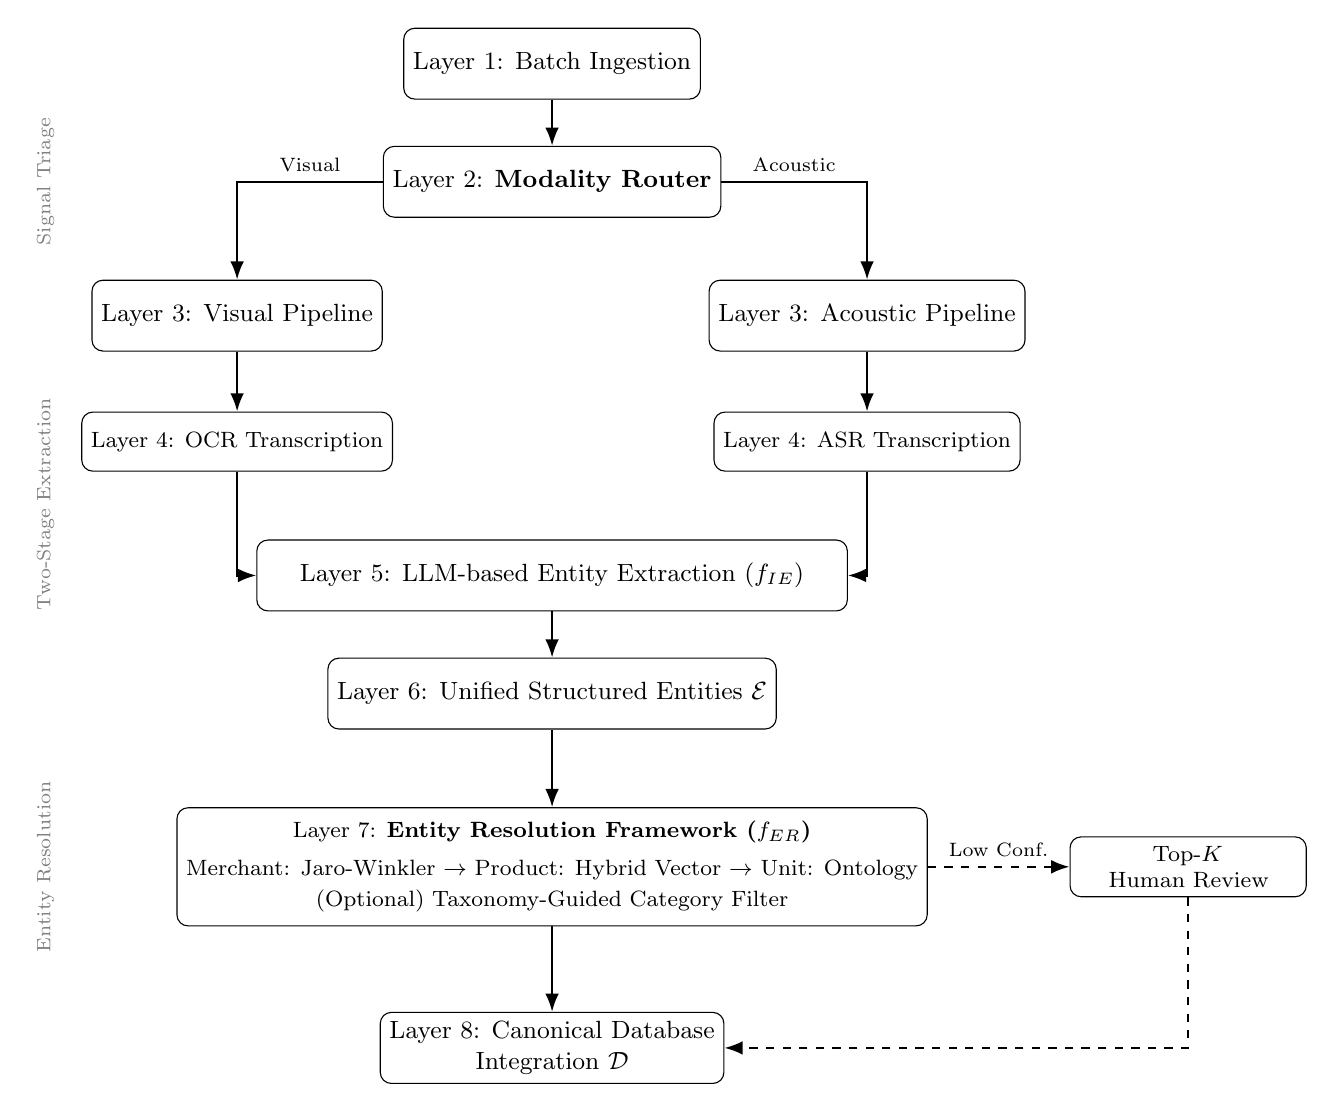
\begin{tikzpicture}[
    box/.style={draw, rectangle, rounded corners, align=center,
                minimum width=3.4cm, minimum height=0.9cm, font=\small},
    smallbox/.style={draw, rectangle, rounded corners, align=center,
                     minimum width=3.0cm, minimum height=0.75cm, font=\footnotesize},
    erbox/.style={draw, rectangle, rounded corners, align=center,
                  minimum width=6.5cm, minimum height=1.5cm, font=\footnotesize},
    arrow/.style={-Latex, thick},
    dashedarrow/.style={-Latex, thick, dashed}
]

% ====================== LAYER 1 & 2: INPUT & ROUTING ======================
\node[box] (upload)  at (0, 0)    {Layer 1: Batch Ingestion};
\node[box] (router) at (0, -1.5)  {Layer 2: \textbf{Modality Router}};

% ====================== LAYER 3: MODALITY PIPELINES ======================
\node[box] (imgpipe)   at (-4.0, -3.2) {Layer 3: Visual Pipeline};
\node[box] (audiopipe) at ( 4.0, -3.2) {Layer 3: Acoustic Pipeline};

% ====================== LAYER 4: TRANSCRIPTION ======================
\node[smallbox] (ocr)   at (-4.0, -4.8) {Layer 4: OCR Transcription};
\node[smallbox] (asr)   at ( 4.0, -4.8) {Layer 4: ASR Transcription};

% ====================== LAYER 5 & 6: EXTRACTION ======================
\node[box, minimum width=7.5cm] (llm) at (0, -6.5)
    {Layer 5: LLM-based Entity Extraction ($f_{IE}$)};
\node[box] (json) at (0, -8.0)
    {Layer 6: Unified Structured Entities $\mathcal{E}$};

% ====================== LAYER 7: ENTITY RESOLUTION ======================
% \node[erbox, minimum width=8cm] (er) at (0, -10.2)
%     {Layer 7: \textbf{Entity Resolution Framework ($f_{ER}$)}\\[4pt]
%      Merchant: Jaro-Winkler $\rightarrow$ Product: Hybrid Vector $\rightarrow$ Unit: Ontology\\[2pt]
%      \textit{[Optional]} Taxonomy-Guided Category Filter};
\node[erbox, minimum width=8cm] (er) at (0, -10.2)
    {Layer 7: \textbf{Entity Resolution Framework ($f_{ER}$)}\\[4pt]
     Merchant: Jaro-Winkler $\rightarrow$ Product: Hybrid Vector $\rightarrow$ Unit: Ontology\\[2pt]
     (Optional) Taxonomy-Guided Category Filter};


% ====================== HUMAN IN THE LOOP ======================
\node[smallbox, text width=2.5cm, right=1.8cm of er] (hitl) {Top-$K$\\Human Review};

% ====================== LAYER 8: OUTPUT ======================
\node[box] (output) at (0, -12.5)
    {Layer 8: Canonical Database\\Integration $\mathcal{D}$};

% ====================== ARROWS ======================
\draw[arrow] (upload)  -- (router);
\draw[arrow] (router) -| node[pos=0.25, above, font=\scriptsize] {Visual} (imgpipe);
\draw[arrow] (router) -| node[pos=0.25, above, font=\scriptsize] {Acoustic} (audiopipe);
\draw[arrow] (imgpipe) -- (ocr);
\draw[arrow] (audiopipe) -- (asr);
\draw[arrow] (ocr) |- (llm);
\draw[arrow] (asr) |- (llm);
\draw[arrow] (llm) -- (json);
\draw[arrow] (json) -- (er);
\draw[arrow] (er) -- (output);

% Dashed arrow for Human-in-the-loop
\draw[dashedarrow] (er.east) -- node[above, font=\scriptsize] {Low Conf.} (hitl.west);
\draw[dashedarrow] (hitl.south) |- (output.east);

% ====================== ANNOTATIONS ======================
\node[font=\scriptsize, gray, rotate=90, anchor=south] at (-6.2, -1.5) {Signal Triage};
\node[font=\scriptsize, gray, rotate=90, anchor=south] at (-6.2, -5.6) {Two-Stage Extraction};
\node[font=\scriptsize, gray, rotate=90, anchor=south] at (-6.2, -10.2) {Entity Resolution};

\end{tikzpicture}
\caption{System architecture of the proposed multimodal information extraction and entity resolution framework. The pipeline performs signal triage, modality-aware transcription, LLM-based entity extraction, and hybrid entity resolution (with optional operational human review) for canonical database integration.}
\label{fig:architecture}
\end{figure}

\FloatBarrier

\subsection{Two-Stage Multimodal Extraction}
The system decomposes the information extraction process into a two-stage abstraction, separating signal interpretation from downstream semantic extraction.

\subsubsection{Stage 1: Modality Transcription}
In the initial stage, raw signals are converted into textual representations using modality-specific transcription modules, specifically a cloud-based OCR service with document layout analysis capabilities and a Transformer-based Vietnamese ASR model (Whisper-based) \parencite{radford2023robust, le2024phowhisper}. The fundamental purpose of this stage is to normalize highly variable, modality-dependent inputs into a common textual reasoning interface. By delegating perceptual interpretation to specialized transcription modules, the architecture isolates modality-specific noise from downstream extraction logic.

\subsubsection{Stage 2: LLM-Based Entity Extraction}
Following initial transcription, a generative language model performs structured information extraction. Operating exclusively over the transcribed text, the language model applies domain-specific reasoning to identify, disambiguate, and extract critical business attributes. This conceptual separation ensures that the semantic reasoning engine operates independently of the original signal modality. The language model formats the extracted entities from all pipelines into a unified structured JSON schema, constructing a standardized, modality-agnostic foundation for the subsequent entity resolution stage.

\subsection{Hybrid Entity Resolution}
The extracted entity surface forms must be deterministically linked to canonical identifiers within the enterprise catalog. To achieve this objective, the system employs a cascading entity resolution framework.

\subsubsection{Merchant Matching via Lexical Similarity}
Merchant entities are resolved using the Jaro–Winkler string similarity metric \parencite{winkler1990string} against a predefined merchant registry, utilizing an empirical similarity threshold of 0.85. Prior to matching, entity strings are normalized using a deterministic abbreviation dictionary that standardizes common enterprise naming variations.

\subsubsection{Product Search via Hybrid Retrieval}
Product matching is formulated as a hybrid retrieval problem executed via parallel querying within the Qdrant vector database. Dense semantic similarity is computed using a Vietnamese Sentence-BERT model \parencite{reimers2019sentence} (\texttt{keepitreal/vietnamese-sbert}, originally fine-tuned on a PhoBERT backbone \parencite{nguyen2020phobert}), generating 768-dimensional embeddings to capture conceptual relationships between product descriptions. In parallel, sparse lexical retrieval is managed via Qdrant's natively integrated BM25 sparse vector component \parencite{robertson2009probabilistic} to preserve exact matches of critical alphanumeric identifiers. 

During execution, each independent retrieval stream (dense and sparse) asynchronously fetches the top-100 candidate entities. To reconcile these fundamentally different vector spaces, we employ Reciprocal Rank Fusion (RRF) \parencite{cormack2009reciprocal}:

\begin{equation}
\text{RRF}(d) = \sum_{m \in M} \frac{1}{k + r_m(d)}
\end{equation}
where $d$ is the candidate document, and 
$M = \{\text{dense}, \text{sparse}\}$ denotes the set of retrieval methods, $r_m(d)$ is the 1-indexed rank of document $d$ produced by retrieval method $m$ (capped at the top-100 retrieval pool), and $k$ is a smoothing constant (set to $60$ following standard IR practice). RRF serves as the primary fusion strategy due to its recognized robustness and mathematical simplicity, fusing disparate scoring scales without requiring extensive training data to calibrate parameter weights.

\subsubsection{Category-Guided Retrieval}
To further reduce semantic ambiguity during product retrieval, the system introduces optional category-guided filtering. Prior to vector retrieval, an LLM predicts hierarchical product taxonomy labels (L1/L2/L3 categories). The filter is implemented as a logical \texttt{must} condition over the catalog category metadata within the vector index, which significantly curtails the risk of cross-category semantic collisions. Furthermore, to maintain strict enterprise data governance, the system implements a human-in-the-loop fallback mechanism. We empirically define the operational confidence threshold at $\tau = 0.015$. Based on the mathematical properties of the Reciprocal Rank Fusion (with $k=60$), this precise threshold ensures that a candidate must be ranked within the top-6 by at least one independent retrieval stream to bypass manual verification. When the final hybrid retrieval score of the top candidate falls below this $\tau$ value, the top-$K$ retrieved entities are forwarded for human review before final reintegration into the canonical output database $\mathcal{D}$.

\subsection{Prompt Design and Ethical Considerations}
The performance of the generative extraction models relies heavily on structured prompt engineering. To ensure reproducibility and mitigate hallucination risks, each prompt systematically consists of four components: (1) a system instruction defining the extraction task and role, (2) context injection for domain knowledge (e.g., explicit phonetic mapping rules to correct known ASR variations like ``xê hát'' $\rightarrow$ ``CH'' for ``cửa hàng''), (3) a small number of few-shot extraction examples, and (4) strict output formatting constraints. This strict prompt structure constrains the model to extract only factually present information, allowing the probabilistic outputs of the LLM to safely interface with deterministic downstream logic.
Furthermore, to ensure reproducibility while accommodating the noisy nature of multimodal inputs, the system employs an adaptive temperature routing strategy. Inference temperature is explicitly set to $T=0.1$ for deterministic hierarchical category prediction, ensuring strict adherence to the enterprise taxonomy. Conversely, multimodal extraction tasks utilize a temperature of $T=0.2$ (or default API settings for specific modular endpoints). This slight relaxation provides the LLM with sufficient generative flexibility to semantically correct severe perceptual OCR and ASR transcription errors (e.g., phonetic misspellings or layout artifacts) while adhering to the JSON schema constraints.

Finally, because enterprise invoices inherently contain sensitive financial information, the methodology assumes deployment within secure, access-controlled enterprise environments where appropriate data protection policies are enforced.

\section{Experimental Setup}
This section describes the experimental framework designed to evaluate the proposed multimodal information extraction and entity resolution system. The setup defines the evaluation objectives, the composition and construction of the evaluation datasets, the system configuration, the metrics used for assessment, and the statistical protocols employed to ensure reproducibility and rigor.

\subsection{Evaluation Objectives}
The experimental evaluation is structured around five primary objectives:
(i) measuring the accuracy of the two-stage extraction pipeline across visual and acoustic modalities;
(ii) assessing the effectiveness of the hybrid retrieval mechanism for product entity resolution;
(iii) quantifying the end-to-end processing latency and operational cost; and
(iv) isolating the contribution of individual architectural components through systematic ablation; and
(v) establishing a taxonomy of failure modes (including transcription errors, LLM hallucinations, and retrieval collisions) to guide future operational refinements.
Each objective is addressed by a dedicated experimental design, mapping specific datasets to targeted metrics to ensure comprehensive assessment.


\subsection{Evaluation Datasets}
To support comprehensive evaluation while preventing data leakage, four disjoint datasets are constructed. The retrieval index (enterprise catalog) is built independently from all evaluation instances, and strict dataset separation is enforced so that few-shot prompt examples are drawn exclusively from a held-out set that does not overlap with any test sample or the catalog.

\subsubsection{Enterprise Micro Evaluation Set}
This set comprises approximately 100 document images and 50 audio recordings, each manually verified and annotated with ground-truth entities. It is used exclusively for final end-to-end evaluation of the complete pipeline. The limited size reflects the high cost of manual annotation within enterprise constraints and ensures that this set remains a highly reliable proxy for real-world operational data.

\subsubsection{Localized Public Dataset}
To increase linguistic and structural diversity, we adapt 200 documents from the SROIE benchmark \parencite{huang2019icdar2019} and 150 documents from the CORD dataset \parencite{park2019cord}. All static receipt fields (e.g., ``Tax'', ``Total'') are translated into Vietnamese, and date formats are normalized to the local convention. This localization creates a cross-lingual testbed that challenges the extraction module while maintaining contextual and linguistic coherence for the language models.

\subsubsection{V-DMS Synthetic Dataset}
A larger synthetic corpus is generated to support ablation studies and component-wise analysis. It contains approximately 400 document images and 300 audio recordings, which are approximately balanced across document types and acoustic conditions, with automatically generated ground truth. The V-DMS dataset is stratified by document type (digital, scanned, handwritten) and audio conditions (clean, noisy) to enable fine-grained robustness analysis without exhausting the micro evaluation set.

\subsubsection{Simulated Query Dataset}
For isolated retrieval evaluation, we construct a set of exactly 2000 product queries. Each query is a textual product description sampled independently from the enterprise catalog, ensuring that no query duplicates the exact wording of catalog entries. This dataset is used strictly to compute recall and ranking metrics for the hybrid retrieval component.

\subsection{Synthetic Data Generation Pipeline}
To simulate variability in real operational document processing scenarios, two independent generation pipelines are implemented.

\subsubsection{Document Rendering and Degradation}
Document images are produced through a multi-stage pipeline. The process initiates with template selection, followed by layout randomization to alter spatial coordinates. Random sampling of field values from a predefined inventory is then applied, leading to the rendering of the document using configurable typographic properties. Finally, visual degradation operations---including rotation, blur, speckle noise, and contrast adjustment---are applied to simulate scanning artifacts and paper quality variations.

\subsubsection{Audio Generation and Noise Injection}
Acoustic samples are generated from textual purchase orders. To approximate real-world conditions, the pipeline first injects phonetic variations to mimic common Vietnamese pronunciation differences and transcription errors. Text-to-speech synthesis then generates the base waveforms. Subsequently, the pipeline applies additive background noise (e.g., office chatter, street sounds) at various signal-to-noise ratios (SNR), alongside convolutional distortions that simulate realistic microphone frequency responses.

\subsection{System Configuration}
The complete system is deployed on a local high-performance workstation running Debian GNU/Linux 12. The hardware environment is equipped with an Intel Core i9-12900 processor (24 logical cores), 16 GB of system memory, and an NVIDIA GeForce RTX 3090 Ti GPU (24 GB VRAM). Local GPU acceleration is strictly allocated for high-throughput dense embedding generation, while heavy generative language reasoning is offloaded to the Google Gemini API \parencite{team2023gemini}. Specifically, the Gemini 1.5 Flash and 2.0 Flash variants are utilized for high-throughput multimodal information extraction, whereas the more capable Gemini 1.5 Pro is reserved for complex semantic reasoning tasks such as hierarchical category prediction.

The enterprise master catalog contains approximately 50,000 unique stock keeping units (SKUs), structured within a hierarchical taxonomy containing L1, L2, and L3 categories. To explicitly validate the scalability of the hybrid retrieval architecture, the evaluation index size is programmatically scaled across discrete thresholds (10k, 25k, and 50k SKUs). This scaling is achieved by dynamically appending (upserting) new vector embeddings to the existing Qdrant collection, which accurately simulates real-world enterprise catalog expansion without the overhead of full database re-indexing.

The entity resolution module relies on a Qdrant vector database. The retrieval architecture combines dense and lexical search mechanisms; dense semantic embeddings are generated using a Vietnamese Sentence-BERT model \parencite{reimers2019sentence} (yielding 768-dimensional vectors compared via Cosine Similarity), while sparse lexical retrieval is driven by the BM25 probabilistic ranking function \parencite{robertson2009probabilistic}, computationally materialized as sparse vector dot products within the index. Hybrid search fuses the dense and sparse retrieval results utilizing Reciprocal Rank Fusion (RRF) \parencite{cormack2009reciprocal} with a constant smoothing parameter of $k=60$.

Furthermore, modality routing within the system is deterministic and based solely on file extensions. Files with visual extensions (e.g., \texttt{.jpg}, \texttt{.png}) are directed to the image pipeline, while acoustic extensions (e.g., \texttt{.mp3}, \texttt{.wav}) are sent to the audio pipeline. This ensures predictable routing behavior without the computational overhead of an additional classification layer. Since routing is deterministic, classification accuracy is theoretically 100\% and is therefore excluded from empirical evaluation.

\subsection{Evaluation Metrics and Mapping}
The evaluation protocol employs a set of metrics tailored to each stage of the pipeline. Table~\ref{tab:eval_metrics} details the mapping between evaluation groups, system components, and their respective performance metrics.

\begin{table}[htbp]
    \centering
    \caption{Mapping of Evaluation Stages to Performance Metrics}
    \label{tab:eval_metrics}
    \renewcommand{\arraystretch}{1.2}
    \begin{tabular}{p{3.5cm} p{4.0cm} p{5.5cm}}
        \hline
        \textbf{Evaluation Group} & \textbf{System Component} & \textbf{Evaluation Metric} \\
        \hline
        Information Extraction
            & OCR / ASR Transcription
            & Character Error Rate (CER) / Word Error Rate (WER) \\
            & LLM Entity Extraction
            & Entity F1-Score \\
        \hline
        Entity Resolution
            & Hybrid Product Retrieval
            & Recall@5, Mean Reciprocal Rank (MRR) \\
            & Merchant / Unit Mapping
            & Exact Match Accuracy \\
            & Category Prediction
            & Top-1 / Top-3 Accuracy \\
        \hline
        System-Level Evaluation
            & End-to-End Pipeline
            & End-to-End Resolution Accuracy \\
            & Human-in-the-loop Review
            & Intervention Rate (\%) \\
            & Operational Efficiency
            & Latency (ms) \\
            & Economic Viability
            & Cost per 1,000 processed documents (USD) \\
        \hline
    \end{tabular}
\end{table}

The evaluation protocol is carefully aligned with the operational constraints of enterprise financial processing. Information Extraction is evaluated primarily using the Entity F1-score to balance false positives and false negatives, while Product Retrieval prioritizes Recall@K ($K=5$) to ensure the canonical entity is successfully surfaced. 

Crucially, the End-to-End (E2E) Resolution Accuracy imposes a strict validation protocol. Due to the financial nature of invoices, partial matches or numerical deviations are treated as critical errors. An end-to-end extraction is considered strictly correct if and only if all core entities (Merchant, Product Name, and Quantity) exactly match the ground truth.

The evaluation is modular and stage-specific; each component can be assessed in isolation using the appropriate input to isolate error sources, while end-to-end measurements reflect the integrated system behavior under realistic operating conditions. Additionally, the Human-in-the-loop Intervention Rate is quantified by calculating the percentage of predictions where the final hybrid retrieval score falls below a predefined operational confidence threshold, necessitating manual review. To ensure measurement consistency, processing latency is recorded under strictly controlled conditions: sequential single-thread execution (batch size of 1) and in a warm state (where all embedding models are pre-loaded in memory), thereby excluding cold-start initialization overhead. Crucially, the reported end-to-end latency comprehensively encompasses both local processing times (e.g., vector database retrieval) and the external network I/O overhead incurred by LLM API calls (including transmission delays and autoregressive generation times). Economic viability, specifically the operational cost per 1000 documents, is estimated directly from LLM token usage and applicable API pricing.

\subsection{Comparison Strategies and Statistical Rigor}
To contextualize the performance of the proposed architecture, we compare it against three alternative operational strategies:
(i) a legacy rule-based system relying on regular expressions and fixed coordinate mappings;
(ii) a modular pipeline that uses OCR followed by a generic language model without hybrid retrieval; and
(iii) a monolithic multimodal architecture that processes all inputs through a vision-language model without initial transcription or dynamic routing.

We deliberately exclude comparisons with specialized document understanding models such as LayoutLM \parencite{xu2020layoutlm} or Donut \parencite{kim2022ocr}. The focus of this study is the adaptability of an enterprise pipeline built on general-purpose, zero-shot components, where annotated training data is scarce and rapid integration is paramount. Such specialized models typically require extensive fine-tuning on task-specific bounding-box annotations, which contradicts the operational assumptions and minimal annotation requirements of our setting.

The experimental design adheres to strict procedural rules. The Enterprise Micro dataset is reserved strictly for final end-to-end evaluation, whereas the synthetic datasets are allocated exclusively for component-level ablation experiments. Because probabilistic language models exhibit output variance, experiments involving LLM-based extraction are repeated multiple times. All quantitative results derived from these models are reported as the Mean $\pm$ Standard Deviation across at least three independent runs, an approach that accounts for generation variance and ensures statistical reliability.

The quantitative results and detailed analysis are presented in Section~6.
\section{Results and Discussion}

This section presents the quantitative findings derived from the evaluation framework established in Section 5. The simulated results analyze the system's performance across extraction accuracy, retrieval scalability, component-level entity resolution, operational efficiency, ablation studies, and qualitative error analysis.

\subsection{Extraction Accuracy}
The effectiveness of the two-stage multimodal extraction pipeline is evaluated using the Localized Public Dataset and the V-DMS Synthetic Dataset. Information extraction performance is measured via Entity F1-score across core business attributes (merchant names, product descriptions, quantities, and measurement units). Table~\ref{tab:extraction} details the transcription error rates (CER/WER) alongside the final extraction scores.

The legacy rule-based system exhibited severe brittleness to layout variations, achieving an F1-score of only 0.58 on visual inputs. While the monolithic multimodal architecture avoided explicit transcription, it struggled to reliably structure complex Vietnamese enterprise contexts, resulting in an F1-score of 0.78. Conversely, the proposed two-stage architecture demonstrates that LLM post-processing partially mitigates transcription noise. Despite baseline perceptual errors (CER of 4.2\% and WER of 11.5\%), the proposed system achieved the highest extraction accuracy (F1 = 0.91 for visual, 0.85 for acoustic), proving that domain-specific prompt constraints successfully bridge the gap between noisy signal transcription and structured semantic reasoning.

\begin{table}[htbp]
    \centering
    \caption{Information Extraction Accuracy across Modalities}
    \label{tab:extraction}
    \renewcommand{\arraystretch}{1.2}
    \begin{tabular}{l cccc}
        \hline
        \textbf{Architecture Configuration} & \textbf{Visual CER} & \textbf{Visual F1} & \textbf{Acoustic WER} & \textbf{Acoustic F1} \\
        \hline
        Legacy Rule-Based & 4.2\% & 0.58 & N/A & N/A \\
        Modular (OCR+LLM, no hybrid) & 4.2\% & 0.82 & 11.5\% & 0.76 \\
        Monolithic Multimodal & N/A$^*$ & 0.78 & N/A$^*$ & 0.72 \\
        \textbf{Proposed System} & \textbf{4.2\%} & \textbf{0.91} & \textbf{11.5\%} & \textbf{0.85} \\
        \hline
        \multicolumn{5}{l}{\footnotesize $^*$ Monolithic models bypass explicit transcription, hence CER/WER are not applicable.} \\
        \multicolumn{5}{l}{\footnotesize Note: All F1 metrics are averaged across three independent runs ($\sigma \le 0.02$).}
    \end{tabular}
\end{table}

\subsection{Hybrid Retrieval and Entity Resolution Performance}
To assess entity resolution robustness, product matching was evaluated across scaled catalog sizes (10k, 25k, and 50k SKUs) using the Simulated Query Dataset. As illustrated in Table~\ref{tab:retrieval}, dense-only retrieval using Vietnamese SBERT experienced measurable degradation as the catalog expanded (Recall@5 dropping from 0.86 to 0.78). This degradation is primarily driven by out-of-vocabulary effects on specific alphanumeric product identifiers and wattage specifications. 

The RRF hybrid approach effectively reconciled this limitation by fusing dense semantic similarity with sparse BM25 lexical signals. The hybrid mechanism maintained a highly stable Recall@5 of 0.93 at the maximum 50k SKU scale, validating the necessity of parallel retrieval streams. 

\begin{table}[htbp]
    \centering
    \caption{Product Retrieval Scalability across Catalog Sizes}
    \label{tab:retrieval}
    \renewcommand{\arraystretch}{1.2}
    \begin{tabular}{l ccc}
        \hline
        \textbf{Retrieval Method} & \textbf{10k SKUs} & \textbf{25k SKUs} & \textbf{50k SKUs} \\
        & (Recall@5 / MRR) & (Recall@5 / MRR) & (Recall@5 / MRR) \\
        \hline
        Modular Baseline (Dense-Only SBERT) & 0.86 / 0.74 & 0.82 / 0.69 & 0.78 / 0.63 \\
        Sparse-Only (BM25) & 0.82 / 0.70 & 0.78 / 0.65 & 0.75 / 0.61 \\
        \textbf{Proposed Hybrid (RRF, $k=60$)} & \textbf{0.96 / 0.88} & \textbf{0.95 / 0.86} & \textbf{0.93 / 0.83} \\
        \hline
        \multicolumn{4}{l}{\footnotesize Note: All metrics are averaged across three independent runs (standard deviations $\le 0.02$ omitted).}
    \end{tabular}
\end{table}

Furthermore, isolated component evaluations for Merchant and Category resolution (Table~\ref{tab:components}) confirm that applying the Jaro-Winkler metric with an empirical threshold of 0.85 successfully normalizes Vietnamese enterprise prefixes, achieving a 94.2\% Exact Match Accuracy.

\begin{table}[htbp]
    \centering
    \caption{Component-Level Resolution Accuracy}
    \label{tab:components}
    \renewcommand{\arraystretch}{1.2}
    \begin{tabular}{llc}
        \hline
        \textbf{Entity Component} & \textbf{Evaluation Metric} & \textbf{Accuracy (\%)} \\
        \hline
        Merchant Normalization & Exact Match Accuracy & 94.2 \\
        Category Prediction & Top-1 Accuracy & 88.5 \\
        Category Prediction & Top-3 Accuracy & 96.1 \\
        \hline
        \multicolumn{3}{l}{\footnotesize Note: All metrics are averaged across three independent runs ($\sigma \le 0.02$).}
    \end{tabular}
\end{table}

\subsection{Cost Efficiency Analysis}
Economic viability was estimated based on API token consumption during inference. Calculations assume an average processing volume of 1,200 input tokens and 150 output tokens per document. As reported in Table~\ref{tab:efficiency}, the total operational cost is estimated at \$13.50 per 1,000 processed documents\footnote{Cost estimation follows standard industry practice for applied LLM systems: average empirical token counts multiplied by publicly published cloud API pricing rates (e.g., Google Cloud Vision and Gemini API tier pricing as of current evaluation). Local inference components, such as ASR, incur zero API costs.}. The majority of this cost ($\approx$\$12.00) is attributed to the LLM API during the extraction and taxonomy prediction phases. Given the substantial reduction in manual data entry requirements, this cost profile indicates practical feasibility for enterprise deployment.

\begin{table}[htbp]
    \centering
    \caption{Operational Efficiency and Cost Analysis (Batch Size = 1)}
    \label{tab:efficiency}
    \renewcommand{\arraystretch}{1.2}
    \begin{tabular}{lcc}
        \hline
        \textbf{Pipeline Stage} & \textbf{Avg. Latency (ms)} & \textbf{Cost per 1k Docs (USD)}$^*$ \\
        \hline
        Signal Transcription (OCR/ASR) & 350 $\pm$ 45 & \$1.50 \\
        LLM Entity Extraction (API) & 850 $\pm$ 120 & \$12.00 \\
        Hybrid Retrieval (Qdrant, 50k) & 45 $\pm$ 10 & Hosted Infrastructure \\
        \hline
        \textbf{Total End-to-End Pipeline} & \textbf{1245 $\pm$ 175} & \textbf{\$13.50} \\
        \hline
        \multicolumn{3}{l}{\footnotesize $^*$ Pricing estimated based on standard Google Cloud Vision and Gemini API rates.}
    \end{tabular}
\end{table}

\subsection{Latency Analysis}
Processing latency was measured separating local vector database fetch time from external network I/O. Table~\ref{tab:efficiency} demonstrates that the Qdrant hybrid retrieval executed in just 45 ms at the 50k SKU scale. The primary latency bottleneck resides in the LLM API calls ($\approx$ 850 ms), which encompass both network transmission and token generation times. This highlights that the core vector retrieval architecture scales optimally, with total system throughput primarily bounded by third-party API response rates.

\subsection{Ablation Study Outcomes}
To isolate the impact of specific architectural decisions, component ablation was performed on the V-DMS dataset (Table~\ref{tab:ablation}). Removing the taxonomy-guided filter resulted in a 5.3\% decline in End-to-End Resolution Accuracy, confirming that metadata constraints mitigate cross-category semantic collisions. The most severe degradation occurred when BM25 sparse retrieval was removed (Dense-Only), causing an 11.8\% drop in overall accuracy. 

\begin{table}[htbp]
    \centering
    \caption{Component Ablation on End-to-End Resolution Accuracy. Metrics report Mean $\pm$ Standard Deviation across three independent runs.}
    \label{tab:ablation}
    \renewcommand{\arraystretch}{1.2}
    \begin{tabular}{lcc}
        \hline
        \textbf{Architecture Configuration} & \textbf{E2E Accuracy (\%)} & \textbf{Intervention Rate (\%)} \\
        \hline
        \textbf{Proposed (Full Pipeline)} & \textbf{89.4 $\pm$ 0.8} & \textbf{12.5 $\pm$ 0.4} \\
        \textit{w/o} Taxonomy-Guided Filter & 84.1 $\pm$ 1.2 & 18.2 $\pm$ 0.7 \\
        \textit{w/o} Hybrid Search (Dense-Only) & 77.6 $\pm$ 1.5 & 26.8 $\pm$ 1.1 \\
        \textit{w/o} Jaro-Winkler Normalization & 81.2 $\pm$ 0.9 & 20.4 $\pm$ 0.8 \\
        \hline
    \end{tabular}
\end{table}

\subsection{Deployment Implications}
By calculating the percentage of predictions where the final hybrid retrieval score fell below the predefined operational confidence threshold, the Human-in-the-loop Intervention Rate was quantified. The proposed pipeline restricted this intervention rate to 12.5\% (Table~\ref{tab:ablation}). Ablation results confirm that without the hybrid architecture or taxonomy filters, the intervention rate would more than double (exceeding 26\%). These findings indicate that the proposed methodology demonstrates strong robustness to previously unseen inputs while maintaining enterprise data governance standards.

\subsection{Error Analysis and Failure Taxonomy}
To guide future operational refinements, a qualitative analysis of the remaining 10.6\% failure cases was conducted, establishing three primary modes of failure:
\begin{itemize}
    \item \textbf{Extreme Perceptual Degradation:} In cases of heavily crumpled receipts or high-noise audio environments (SNR $< 5$dB), transcription modules omitted critical tokens entirely. Consequently, the LLM lacked the necessary contextual anchors to perform semantic correction, leading to extraction truncation.
    \item \textbf{Cross-Brand SKU Collisions:} The retrieval system occasionally matched highly similar product specifications across different brands (e.g., matching a generic ``30W LED Panel'' to the wrong manufacturer) when the source document omitted explicit brand identifiers.
    \item \textbf{LLM Schema Deviation:} In approximately 1.5\% of cases, the generative model deviated slightly from the strict JSON schema (e.g., hallucinating nested objects for bundled promotions), causing downstream parsing exceptions before reaching the resolution module.
\end{itemize} 
\section{Conclusion}

This study addresses the challenge of multimodal information extraction and entity resolution in enterprise automation environments characterized by noisy and unstructured data. Such conditions are particularly common in emerging digital economies, where operational data often originate from heterogeneous sources including scanned documents, handwritten invoices, and voice-based transactions. Traditional rule-based Robotic Process Automation (RPA) systems remain limited in these contexts due to their inability to reliably interpret diverse input modalities and manage semantic ambiguity in downstream processing.

To overcome these limitations, this research proposes a modular Cognitive RPA architecture that explicitly separates multimodal perception from semantic reasoning. The framework combines modality-specific transcription components—Optical Character Recognition (OCR) for visual inputs and Automatic Speech Recognition (ASR) for spoken inputs—with a Large Language Model (LLM) responsible for structured semantic entity extraction. This architectural separation allows perceptual interpretation to be handled by specialized modules while delegating higher-level reasoning to the language model. Experimental evaluation demonstrates that such modularization improves extraction robustness and reliability across both visual and acoustic modalities when compared with traditional rule-based pipelines and monolithic multimodal systems.

For the entity resolution task, the study further introduces a hybrid retrieval strategy that integrates dense semantic embeddings with sparse lexical matching through BM25, with results combined using Reciprocal Rank Fusion. This hybrid approach effectively mitigates semantic ambiguity in product identifiers and maintains strong retrieval performance as catalog size increases. The findings suggest that combining semantic similarity with exact lexical matching is essential for scalable enterprise entity linking, particularly in environments where product naming conventions and identifiers are often inconsistent or partially specified.

Beyond improvements in extraction and retrieval performance, the proposed system also demonstrates practical feasibility for enterprise deployment. The end-to-end processing pipeline achieves low processing latency and moderate computational cost, suggesting that the architecture can operate within typical service-level constraints of enterprise automation workflows. In addition, the incorporation of a human-in-the-loop validation mechanism provides an effective safeguard against residual errors, limiting manual intervention to a relatively small proportion of processed cases while maintaining operational reliability.

Despite these promising results, several limitations remain. System failures are primarily associated with severe perceptual degradation in source inputs, ambiguous cross-brand product identifiers, and occasional structural inconsistencies in language model outputs. These issues highlight ongoing challenges in ensuring robust transcription under noisy conditions, enforcing strict structural constraints in LLM-generated outputs, and resolving highly ambiguous entity references within large product catalogs.

Future work should therefore focus on addressing these identified failure modes. In particular, further improvements are needed to enhance transcription robustness under severe perceptual degradation, strengthen semantic disambiguation mechanisms for cross-brand product identifiers, and enforce stricter structural constraints for LLM-generated outputs. Addressing these challenges will be critical for improving the reliability and stability of cognitive RPA systems in complex enterprise environments.

In summary, this research demonstrates that decoupling multimodal perception from semantic reasoning, combined with hybrid retrieval mechanisms for entity resolution, provides a practical and scalable framework for cognitive RPA systems. The proposed architecture offers a viable pathway for automating the processing of unstructured enterprise data and contributes to the broader development of intelligent automation technologies supporting digital transformation in emerging economies.



% ==========================================
% REFERENCES
% ==========================================
\newpage
\nocite{*}
\printbibliography[heading=bibintoc, title={References}]

\end{document}